\documentclass[titlepage]{article}

\usepackage{cite}
\usepackage{amsmath}
\usepackage[pdftex]{graphicx}
    \graphicspath{{../figures/}}
    \DeclareGraphicsExtensions{.pdf,.jpg,.png}
\usepackage[hidelinks]{hyperref}
\usepackage[margin=1.0in]{geometry}
\usepackage{placeins}
\usepackage{url}
\usepackage{enumerate}
\usepackage{algorithm}      % to wrap code in an algorithm environment
\usepackage{algpseudocode}  % to use algorithmic env. to write pseudocode
    % new definitions
    \algnewcommand\algorithmicswitch{\textbf{switch}}
    \algnewcommand\algorithmiccase{\textbf{case}}
    % new environments
    \algdef{SE}[SWITCH]{Switch}{EndSwitch}[1]%
        {\algorithmicswitch\ #1\ \algorithmicdo}%
        {\algorithmicend\ \algorithmicswitch}
    \algdef{SE}[CASE]{Case}{EndCase}[1]%
        {\algorithmiccase\ #1}%
        {\algorithmicend\ \algorithmiccase}
\usepackage{booktabs}

\begin{document}

\title{Booth multiplier algorithm specification and FPGA implementation}
\author{Luis M. Gallegos C.}
\date{September 2014}
\maketitle

\begin{abstract}
    This work presents an FPGA implementation of a Booth multiplier, tested in an Atlys Spartan-6 FPGA Trainer Board.
    The work was originally done for an embedded systems class project.
\end{abstract}

%%%%%%%%%%%%%%%%%%%%%%%%%%%%%%%%%%%%%%%%%%%%%%%%%%%%%%%%%%%%%%%%%%%%%%%%%%%%%%%
%                             BRIEF INTRODUCTION                              %
%%%%%%%%%%%%%%%%%%%%%%%%%%%%%%%%%%%%%%%%%%%%%%%%%%%%%%%%%%%%%%%%%%%%%%%%%%%%%%%
\section{Brief introduction} % (fold)
\label{sec:brief_introduction}

The algorithm was developed by Andrew D. Booth and published for the first time in an article in \emph{The Quarterly Journal of Mechanics and Applied Mathematics} in 1951 \cite{Booth1951Signed}.
The algorithm was developed in a time where calculators were faster doing shift operations than sums.\par

% section brief_introduction (end)



%%%%%%%%%%%%%%%%%%%%%%%%%%%%%%%%%%%%%%%%%%%%%%%%%%%%%%%%%%%%%%%%%%%%%%%%%%%%%%%
%                            ALGORITHM DESCRIPTION                            %
%%%%%%%%%%%%%%%%%%%%%%%%%%%%%%%%%%%%%%%%%%%%%%%%%%%%%%%%%%%%%%%%%%%%%%%%%%%%%%%
\section{Algorithm description} % (fold)
\label{sec:algorithm_description}

The main idea behind the algorithm was to reduce the number of sums, considering a sequence of 1s can be represented as a subtraction, as show in \eqref{eq:ones}.
\begin{equation}
    \label{eq:ones}
    1111 = 10000 - 1
\end{equation}\par

Considering this, a multiplication by a sequence of $n$ 1s can be performed with a subtraction, instead of a series of $n$ sums, one for each 1 in the sequence.
See \eqref{eq:multiplication-ones}
\begin{equation}
    \label{eq:multiplication-ones}
    a \times 1111 = a \times \left( 10000 - 1 \right) = a \times 10000 - a
\end{equation}\par

To illustrate the algorithm, we consider $a$ and $x$ the multiplicand and multiplier, respectively, and $p$ the result, all represented in two's complement.
Both $a$ and $x$ are $n = 4$-bit long, with $p$ being 8-bit, all including the sign bit.\par

The algorithm goes through each bit in the multiplier, $x_i$, from LSB to MSB, analyzing each bit and its adjacent $x_{i-1}$, where $i$ goes from $0$ to $n-1$.
For the case of $x_0$, $x_{i-1} = 0$.
Partial sums are performed and their results stored in $p$, where the final result is also stored in the end.
In each iteration, one of four operations is performed, depending on the pair of bits being analyzed:
\begin{enumerate}[a)]
    \item If $x_i = 0$, $x_{i-1} = 0$
        \begin{itemize}
            \item Perform an arithmetic right shift on $p$.
        \end{itemize}
    \item If $x_i = 1$, $x_{i-1} = 1$
        \begin{itemize}
            \item Perform an arithmetic right shift on $p$.
        \end{itemize}
    \item If $x_i = 0$, $x_{i-1} = 1$
        \begin{itemize}
            \item Add $a$ to $p$, in its most significant half.
            \item Perform an arithmetic right shift on $p$.
        \end{itemize}
    \item If $x_i = 1$, $x_{i-1} = 0$
        \begin{itemize}
            \item Subtract $a$ from $p$, in its most significant half.
            \item Perform an arithmetic right shift on $p$.
        \end{itemize}
\end{enumerate}\par

To make operations easier, the following values are defined.\par

\begin{table}[ht]
    \caption{Additional values for the procedure.}
    \label{tab:values}
    \centering
    \begin{tabular}{cl}
        \toprule
        Values & Description \\
        \midrule
        $\bar{a}$ & $a$'s two's complement \\
        $A$       & $ \{ a , 0000 \}$ ($a$ concatenated with $n$ zeros) \\
        $\bar{A}$ & $ \{ \bar{a} , 0000 \}$ ($\bar{a}$ concatenated with $n$ zeros) \\
        \bottomrule
    \end{tabular}
\end{table}

The reason for $A$ is to be able to add $a$ to $p$ in its most significant half.
Likewise, the reason for $\bar{A}$ is to subtract $a$ from $p$ in its most significant half, through a sum with the two's complement of $a$ (opposite sign).\par

Algorithm~\ref{alg:booth-implementation} shows the algorithm for the implementation.

\begin{algorithm}
    \caption{Booth implementation algorithm}
    \label{alg:booth-implementation}
    \begin{algorithmic}[1]
        \State{$\bar{a} \gets -a$}
        \State{$A \gets \{ a , 0000 \}$}
        \State{$\bar{A} \gets \{ -a, 0000 \}$}
        \State{$p \gets 0000~0000$}
        \State{$i \gets 0$}
        \For{$i = 0$ \textbf{to} $n-1$}
            \Switch{$x_i$, $x_{i-1}$}\Comment{Analyze $x_i$ and $x_{i-1}$}
                \Case{$0,0$}
                    \State{$p \gets p >>> 1$}
                \EndCase
                \Case{$1,1$}
                    \State{$p \gets p >>> 1$}
                \EndCase
                \Case{$0,1$}
                    \State{$p \gets p + A$}\Comment{Ignore overflow}
                    \State{$p \gets p >>> 1$}
                \EndCase
                \Case{$1,0$}
                    \State{$p \gets p + \bar{A}$}\Comment{Ignore overflow}
                    \State{$p \gets p >>> 1$}
                \EndCase
            \EndSwitch
        \EndFor
    \end{algorithmic}
\end{algorithm}

% section algorithm_description (end)



%%%%%%%%%%%%%%%%%%%%%%%%%%%%%%%%%%%%%%%%%%%%%%%%%%%%%%%%%%%%%%%%%%%%%%%%%%%%%%%
%                                   EXAMPLE                                   %
%%%%%%%%%%%%%%%%%%%%%%%%%%%%%%%%%%%%%%%%%%%%%%%%%%%%%%%%%%%%%%%%%%%%%%%%%%%%%%%
\section{Example} % (fold)
\label{sec:example}

For this example, we have the following values for multiplicand $a$ and multiplier $x$.

\begin{table}[ht]
    \centering
    \begin{tabular}{ccc}
        \toprule
        Variable & Binary value & Decimal value \\
        \midrule
        $a$ & 1011 & -5 \\
        $x$ & 1010 & -6 \\
        \bottomrule
    \end{tabular}
\end{table}

From $a$ and $x$, we get:
\begin{align*}
    \bar{a} &= 0101 \\
    A &= 1011 0000 \\
    \bar{A} &= 0101 0000
\end{align*}\par

Additionally, $p$ is initialized, $p = 0000~0000$.\par

The bits from $x$ can now be analyzed.
The following is a step by step execution of the algorithm.\par

\begin{table}[ht]
    \centering
    \begin{tabular}{rrl}
        \multicolumn{3}{c}{$\mathbf{x_0 = 0}$, $\mathbf{x_{-1} = 0}$} \\
        \midrule
        $p = p>>>1 =$ & $0000~0000$ & \\[15pt]


        \multicolumn{3}{c}{$\mathbf{x_1 = 1}$, $\mathbf{x_0 = 0}$} \\
        \midrule
                            &             $0000~0000$  & $p$ \\
                            & $\underline{+0101~0000}$ & $\bar{A}$ \\
        $p = p + \bar{A} =$ &             $0101~0000$  & \\[10pt]
        $p = p>>>1 =$       & $0010~1000$ & \\[15pt]


        \multicolumn{3}{c}{$\mathbf{x_2 = 0}$, $\mathbf{x_1 = 1}$} \\
        \midrule
        \multicolumn{3}{c}{$p = p + A$} \\
                      &             $0010~1000$  & $p$ \\
                      & $\underline{+1011~0000}$ & $A$ \\
        $p = p + A =$ &             $1101~1000$  & \\[10pt]
        $p = p>>>1 =$ & $1110~1100$ & \\[15pt]


        \multicolumn{3}{c}{$\mathbf{x_3 = 1}$, $\mathbf{x_2 = 0}$} \\
        \midrule
        \multicolumn{3}{c}{$p = p + \bar{A}$} \\
                            &             $1110~1100$  & $p$ \\
                            & $\underline{+0101~0000}$ & $\bar{A}$ \\
        $p = p + \bar{A} =$ &          $(1)0011~1100$  & \\
                            & \footnotesize{ignore overflow (1)} & \\[10pt]
        $p = p>>>1 =$       & $0001~1110$ & \\
    \end{tabular}
\end{table}

\FloatBarrier

At the end of the operations, we have a final value of $p = 0001~1110$, which is $30$ in decimal notation, the correct answer for the multiplication $-5 \times -6 = 30$.\par

\figurename~\ref{fig:booth-multiplier-sim} shows the result of this same operation in the ISE simulator.

\begin{figure}[ht]
    \centering
    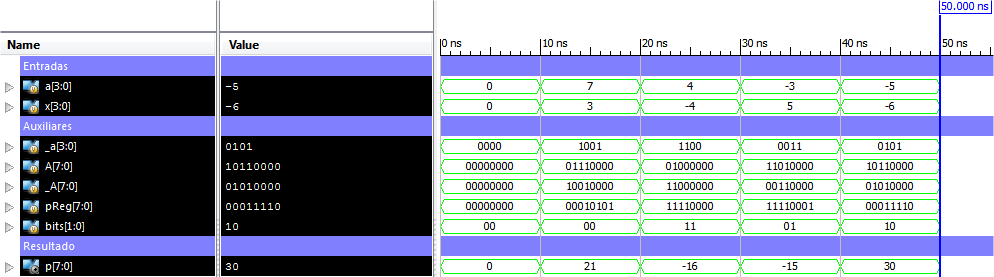
\includegraphics[width=0.75\textwidth]{booth-multiplier-sim}
    \caption{Booth multiplier simulation.}
    \label{fig:booth-multiplier-sim}
\end{figure}

% section example (end)



%%%%%%%%%%%%%%%%%%%%%%%%%%%%%%%%%%%%%%%%%%%%%%%%%%%%%%%%%%%%%%%%%%%%%%%%%%%%%%%
%                               IMPLEMENTATION                                %
%%%%%%%%%%%%%%%%%%%%%%%%%%%%%%%%%%%%%%%%%%%%%%%%%%%%%%%%%%%%%%%%%%%%%%%%%%%%%%%
\section{Implementation} % (fold)
\label{sec:implementation}

The algorithm was implemented in an Atlys Spartan-6 FPGA Trainer Board \cite{AtlysWeb}.
The 4-bit multiplier $x$ is input using switches SW7-SW4, where SW4 is the LSB.
The 4-bit multiplicand $a$ is input using switches SW3-SW0, where SW0 is the LSB.
The 8-bit product $p$ is displayed with the LEDs LD7-LD0, where LD0 is the LSB.
These specifications can be seen in the \emph{ucf} implementation file.\par

A short video showing the multiplier functioning on the Atlys board can be seen in the link \url{http://youtu.be/RQSdaQeM46E}~\cite{Gallegos2014Multiplicador}.

% section implementation (end)



%%%%%%%%%%%%%%%%%%%%%%%%%%%%%%%%%%%%%%%%%%%%%%%%%%%%%%%%%%%%%%%%%%%%%%%%%%%%%%%
%                                BIBLIOGRAPHY                                 %
%%%%%%%%%%%%%%%%%%%%%%%%%%%%%%%%%%%%%%%%%%%%%%%%%%%%%%%%%%%%%%%%%%%%%%%%%%%%%%%
\bibliographystyle{IEEEtran}
\bibliography{IEEEabrv,bibliography}



\end{document}
